% Document formating
\documentclass[12pt]{article}
\setlength{\parindent}{0pt}
\setlength{\oddsidemargin}{0in}
\setlength{\evensidemargin}{0in}
\setlength{\textwidth}{6.5in}
\setlength{\parskip}{\baselineskip}
\usepackage{amsmath,amsfonts,amssymb,wasysym}
\setlength{\evensidemargin}{1in}
\addtolength{\evensidemargin}{-1in}
\setlength{\oddsidemargin}{1.5in}
\addtolength{\oddsidemargin}{-1.5in}
\setlength{\topmargin}{1in}
\addtolength{\topmargin}{-1.5in}
\setlength{\textwidth}{16cm}
\setlength{\textheight}{23cm}
\setlength{\parskip}{0.75cm}

% Brackets
\usepackage{mathtools}
\DeclarePairedDelimiter\ceil{\lceil}{\rceil}
\DeclarePairedDelimiter\floor{\lfloor}{\rfloor}

% Typesetting options
\usepackage{fancyvrb}
\usepackage{tgbonum}
\usepackage{amsmath,amsfonts,amssymb}
\usepackage [english]{babel}
\usepackage [autostyle, english = american]{csquotes}
\MakeOuterQuote{"}
\usepackage{upquote}
\usepackage{scrextend}
\addtokomafont{labelinglabel}{\sffamily}
\usepackage[none]{hyphenat}
\usepackage{url}
\newcommand\tab[1][1cm]{\hspace*{#1}} %creates tab command (~5 spaces)

% Tikz settings
\usepackage{tikz}
\usetikzlibrary{trees}
\usetikzlibrary {positioning}
\definecolor {mypurple}{cmyk}{0.6,0.4,0.1,0}
\definecolor {myred}{cmyk}{0,0.3,0.3,0}
\usetikzlibrary{fit,shapes.misc}

% Fancy font
\usepackage{amsmath}
\usepackage{mathrsfs}
\DeclareMathAlphabet{\mathscrbf}{OMS}{mdugm}{b}{n}

% Other math tools
\usepackage{mathtools}

% Other useful options
\usepackage[table]{colortbl}

% Other graphics
\graphicspath{{PS 7/}}

% Links
\usepackage{hyperref}
\hypersetup{
    colorlinks=true,
    linkcolor=blue,
    filecolor=magenta,      
    urlcolor=cyan,
}
 
\urlstyle{same}

% Code colorering
\usepackage{listings}
\usepackage{color}
\definecolor{codegreen}{rgb}{0,0.6,0}
\definecolor{codegray}{rgb}{0.5,0.5,0.5}
\definecolor{codepurple}{rgb}{0.58,0,0.82}
\definecolor{backcolour}{rgb}{0.95,0.95,0.92}
\lstdefinestyle{mystyle}{
    backgroundcolor=\color{backcolour},   
    commentstyle=\color{codegreen},
    keywordstyle=\color{blue},
    numberstyle=\tiny\color{codegray},
    stringstyle=\color{codepurple},
    basicstyle=\footnotesize,
    breakatwhitespace=false,         
    breaklines=true,                 
    captionpos=b,                    
    keepspaces=true,                 
    numbers=left,                    
    numbersep=5pt,                  
    showspaces=false,                
    showstringspaces=false,
    showtabs=false,                  
    tabsize=2
}
\lstset{style=mystyle}

% --------------------------------
\begin{document}

% ------------- HEADER -----------
CSCI 3104, Fall 2017 \hfill Final Exam\\
John Letey (12/11) \hfill john.letey@colorado.edu\vspace{-11mm}

\hrulefill

{\fontfamily{cmr}\selectfont\vspace{-8mm}
% ##################  PROBLEM 1 #####################
\section*{{\fontfamily{qcr}\selectfont Problem 1 (20 points)}}\vspace{-10mm}
\textsl{Given an array $\{a_1, a_2, \cdots; a_n\}$, a reverse is a pair $(a_i, a_j)$ such that $i < j$ but $a_i > a_j$. Design a divide-and-conquer algorithm with a run-time of $\mathcal{O}(n\log(n))$ for computing the number of reverses in the array. Your solution to this question needs to include both a written explanation and a Python implementation of your algorithm, including:}
\begin{enumerate}
% ----------------------------  PART 1A  -----------------------------------
\item[(a)]\textsl{Explain how your algorithm works, including pseudocode.}\\ \\
The run-time of this algorithm has to be $\mathcal{O}(n\log(n))$, and the algorithm has to be a divide-and-conquer algorithm, so I took a hint and decided to build my algorithm off of the Merge-Sort Algorithm (since it has both the run-time requirement and the algorithm type requirement). Thus, I'm going to have use the same reasoning as the Merge-Sort Algorithm. Here is the pseudocode for the Merge-Sort Algorithm (note that this pseudocode was taken from the book):
\begin{lstlisting}
// The Merge-Sort Algorithm
Merge-Sort(A, p, r)
  if p < r
    q = floor((p + r)/2)
    Merge-Sort(A, p, q)
    Merge-Sort(A, q + 1, r)
    Merge(A, p, q, r)
\end{lstlisting}
I have to modify the above pseudocode for the function \texttt{Merge-Sort} to be able to return the number of reverses in the array. I will also modify the pseudocode for the Merge procedure. Here is some pseudocode (also taken from the book) for the Merge procedure:
\begin{lstlisting}
// The merge procedure
Merge(A, p, q, r)
  n1 = q - p + 1
  n2 = r - q
  let L[1 ... n1+1] and R[1 ... n2+1] be new arrays
  for i = 1 to n1
    L[i] = A[p + i - 1]
  for j = 1 to n2
    R[j] = A[q + j]
  L[n1 + 1] = infinity
  R[n2 + 1] = infinity
  i = 1
  j = 1
  for k = p to r
    if L[i] <= R[j]
      A[k] = L[i]
      i = i + 1
    else 
      A[k] = R[j]
      j = j + 1
\end{lstlisting}
The pseudocode for the \texttt{Merge} procedure won't need a lot of changes. All I need to do is add a counter for it to return. I will also be getting rid of lines 8 and 9 of the pseudocode.
% ----------------------------  PART 1B  -----------------------------------
\item[(b)]\textsl{Implement your algorithm in Python.}\\ \\
Here is my Python code, which is also included in \texttt{Letey-John-Final.py}:
\begin{lstlisting}[language=Python]
## Implementation of Count
def Count(A, p, q, r):
  # Initialize the variable that will hold the number of reverses in 
  # the array A[p:r]
  count = 0
  # Define the size of the left half and right half of the array A[p:r]
  n1 = q - p + 1
  n2 = r - q
  # Calculate the left half and the right half of the array A[p:r]
  L = []
  R = []
  for i in range(n1):
    L.append(A[p + i])
  for j in range(n2):
    R.append(A[q + j + 1])
  # Define some indeces
  i, j, k = 0, 0, p
  # Calculate the number of reverses in the array A[p:r]
  while i < n1 and j < n2:
    if L[i] <= R[j]:
      A[k] = L[i]
      i += 1
    else:
      A[k] = R[j]
      j += 1
      count += (n1 - i)
    k += 1
  # Return the number of reverses in the array A[p:r]
  return count
## Implementation of CountReverses
def CountReverses(A, p, r):
  # Initialize the variable that will hold the number of reverses in
  # the array A[p:r]
  count = 0
  # Calculate the number of reverses in the array A[p:r]
  if p < r:
    q = math.floor((p + r)/2)
    count += CountReverses(A, p, q)
    count += CountReverses(A, q+1, r)
    count += Count(A, p, q, r)
  # Return the count of reverses in the array A[p:r]
  return count
\end{lstlisting}
% ----------------------------  PART 1C  -----------------------------------
\item[(c)]\textsl{Randomly generate an array of 100 numbers and use it as input to run your code. Report on both the input to your code and on how the output demonstrates the correctness of your algorithm.}\\ \\
For the input \texttt{[79, 48, 100, 89, 52, 5, 61, 56, 71, 57, 4, 97, 72, 98, 4, 24, 19, 96, 96, 73, 63, 61, 57, 9, 85, 24, 39, 2, 36, 18, 32, 0, 21, 53, 73, 9, 90, 81, 82, 0, 69, 92, 39, 62, 57, 46, 6, 97, 56, 24, 88, 15, 21, 13, 70, 40, 11, 3, 23, 72,95, 66, 49, 53, 74, 33, 14, 45, 32, 14, 47, 2, 47, 86, 83, 32, 63, 7, 5, 74, 10, 64, 93, 64, 33, 37, 34, 65, 52, 89, 64, 8, 15, 64, 48, 44,45, 8, 6, 48]}, there are 2713 reverses.
\end{enumerate}
% ====================================

% ##################  PROBLEM 2 #####################
\section*{{\fontfamily{qcr}\selectfont Problem 2 (25 points)}}\vspace{-10mm}
\textsl{Suppose that you are assigned a task to do a survey about $n$ important issues (such as education policy and health insurance mandate), by asking a group of $m$ persons questions about these issues. Suppose that a person may not have an opinion about all the issues, and you can ask a person about an issue only if s/he has an opinion about it. We use a bipartite graph $G = \{P \cup I, E\}$ to capture whether a person $p \in P$ has an opinion about an issue $i \in I$ or not: $(p, i) \in E$ means that $p$ has an opinion about $i$. For each issue $i$, in order to have a reliable survey you need to ask at least $l_i$ persons about it, but you may have certain budget constraint so that you can only ask at most $u_i$ persons about it. For each person $p$, you may ask her/him between $b_p$ and $t_p$ issues.}\\ \\
\textsl{Given $G$ and parameters $(l_i, u_i), i \in I$ and $(b_p, t_p), p \in P$, design an algorithm to determine if these parameters are feasible, by formulating it as a problem of finding a routing with lower bounds as in Problem 1 of homework set \#9. You shall solve the problem according to the following steps.}
\begin{enumerate}
% ----------------------------  PART 2A  -----------------------------------
\item[(a)]\textsl{Show how to formulate the parameter feasibility problem as a problem of finding a routing with lower bounds. The resulting problem should be specified by certain graph $G' = \{V', E'\}$ with capacity $c(e)$ and lower bound $l(e)$ for each edge $e \in E'$ and demand $r(v)$ at each vertex $v \in V'$.}\\ \\
% ----------------------------  PART 2B  -----------------------------------
\item[(b)]\textsl{Further formulate the problem as a maximum flow problem as in Problem 1 of homework set \#9. The resulting problem should be specified by certain graph $\hat{G} = \{\hat{V}, \hat{E}\}$ with source $s$, sink $t$ and capacity $c(e)$ for each edge $e \in \hat{E}$.}\\ \\
% ----------------------------  PART 2C  -----------------------------------
\item[(c)]\textsl{Implement $(a)-(b)$ in Python. Your code should take the graph $G$ and parameters $(l_i, u_i), i \in I$ and $(b_p, t_p), p \in P$ as the input, and produce the graph $\hat{G}$ with source $s$, sink $t$ and capacity $c(e), e \in \hat{E}$ as the output.}\\ \\
Here is my Here is my Python code, which is also included in \texttt{Letey-John-Final.py}:
\begin{lstlisting}[language=Python]
## Implementation of calculateHatGraph
def calculateHatGraph(G, bptp, liui):
  # Define another graph to G
  GHat = G
  # Add a super source and a super sink to the graph
  GHat.add_nodes_from(['S', 'T'])
  # Define indeces
  personIndex, issueIndex = 0, 0
  # Add lower bounds
  for node in list(GHat.nodes()):
    if node[:5] == 'Issue':
      if issueIndex < len(liui):
        GHat.add_edge(node, 'T', lower=liui[issueIndex][0], capacity=liui[issueIndex][1])
        issueIndex += 1
    else:
      if personIndex < len(bptp):
        GHat.add_edge('S', node, lower=bptp[personIndex][0], capacity=bptp[personIndex][1])
        personIndex += 1
  # Return the new graph
  return GHat
\end{lstlisting}
% ----------------------------  PART 2D  -----------------------------------
\item[(d)]\textsl{Further implement the Ford-Fulkerson Algorithm in Python to find the maximum flow from $s$ to $t$ over the graph $\hat{G}$.}\\ \\
% ----------------------------  PART 2E  -----------------------------------
\item[(e)]\textsl{Generate a test case of parameters according to the following specifications, and run your code to see if the parameters generated are feasible.}
\begin{itemize}
  \item \textsl{The number of issues $n = 10$ and the number of person $m = 1000$;}
  \item \textsl{For any person $p$ and for any issue $i$, s/he has a probability of 50\% to have an opinion about the issue, i.e., there is a 50\% probability that there is a link from $p$ to $i$ in the graph $G$;}
  \item \textsl{For any person $p$, denote $h_p$ the number of issues that s/he has an opinion about. Let $b_p = \floor{h_p/2}$ and $t_p = h_p$.}
  \item \textsl{For each issue $i$, $l_i$ is drawn uniformly from the interval [300, 400] and $u_i$ uniformly from [500, 700]}
\end{itemize}
\end{enumerate}
% ====================================

% ##################  PROBLEM 3 #####################
\section*{{\fontfamily{qcr}\selectfont Problem 3 (10 points)}}\vspace{-10mm}
\textsl{Suppose you have been sent back in time and have arrived at the scene of an ancient Roman battle. It is your job to assign $n$ spears to $n$ Roman soldiers so that each soldier has a spear. It is best if your assignments minimize the difference in heights between the height of the man and the height of his spear. That is, if the $i^{th}$ man has height $m_i$, and his spear has height $s_i$, then you want to minimize: $\sum_{i} \left| ~ m_i - s_i ~ \right|$}
\begin{enumerate}
% ----------------------------  PART 3A  -----------------------------------
\item[(a)]\textsl{Design algorithm to find the optimal, or near optimal, solution without evaluating all possible combinations. Include an explanation and pseudocode showing how your algorithm works.}\\ \\
\begin{lstlisting}
findOptimalSolution(spears, soldiers) {
  spears = Merge-Sort(spears) // Sort the spears using mergesort
  soldiers = Merge-Sort(soldiers) // Sort the spears using mergesort
  pairs = new list of length n
  for i = 0 to n {
    pairs[i] = (soldiers[i], spears[i])
  }
  return pairs
}
\end{lstlisting}
% ----------------------------  PART 3B  -----------------------------------
\item[(b)]\textsl{Compare the runtime complexity of your algorithm with the complexity of a brute force solution.}\\ \\
The brute force solution for this algorithm would have a runtime of $\mathcal{O}(n^2)$, since you'd go through every possible combination. My algorithm on the other hand, is $n\log(n) + n\log(n) + n$, which is $\mathcal{O}(n\log(n))$, which is way better than $\mathcal{O}(n^2)$.
\end{enumerate}
% ====================================

% ##################  PROBLEM 4 #####################
\section*{{\fontfamily{qcr}\selectfont Problem 4 (20 points)}}\vspace{-10mm}
\textsl{Consider the following spider-web graph that shows a spider siting at the bottom of its web, and a fly sitting at the top. On moodle, there is a file called graphExample.py that implements the graph using a library called NetworkX.}
\begin{center}
  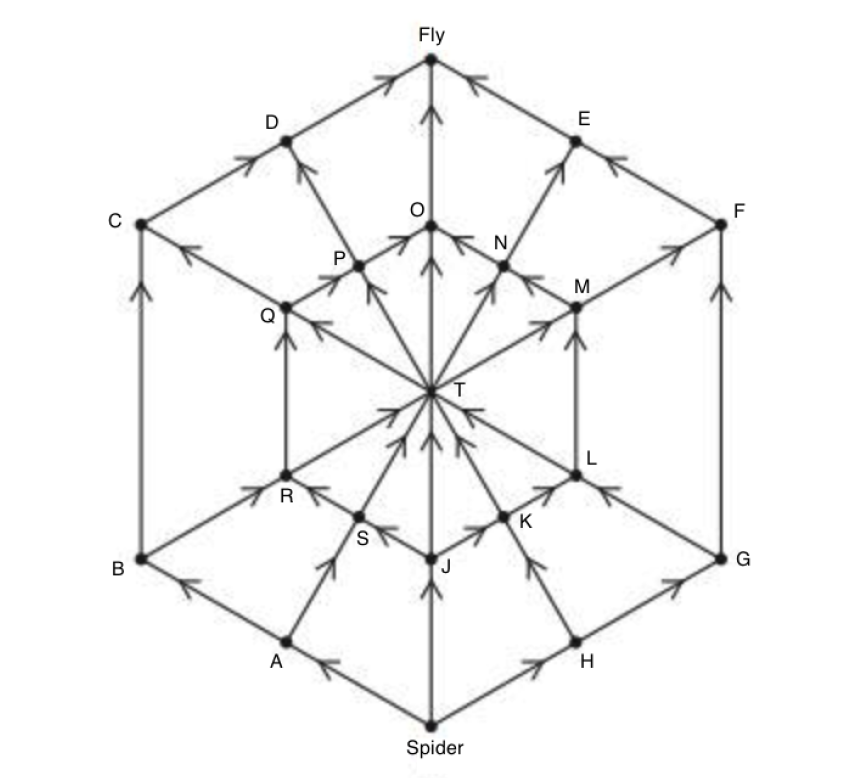
\includegraphics[scale=0.4]{Web.png}
\end{center}
\begin{enumerate}
% ----------------------------  PART 4A  -----------------------------------
\item[(a)]\textsl{Write an algorithm to determine how many different ways can the spider reach the fly by moving along the web’s lines in the directions indicated by the arrows?}\\ \\
I am going to use recursion for this algorithm. My algorithm will start off by getting all of the predecessor nodes to the target (predecessors are the nodes that you can go to the target from). If any of those predecessor nodes happen to be the source, my algorithm will return 1, since there's exactly one path that goes from the source to the target. Else, it will go through each of the predecessors and count how many paths there are from the source to that predecessor (thus, recursion). My algorithm will return the sum of the counts that each of the recursive calls returned.
% ----------------------------  PART 4B  -----------------------------------
\item[(b)]\textsl{Implement your algorithm in Python using the NetworkX graph provided as your data structure. You may need to install NetworkX if it isn’t part of your Python installation. Do not use any of the NetworkX features that would make this problem trivial as part of your solution. However, you can use anything in NetworkX to verify your solution. Your algorithm should return an answer to the question in part (a).}\\ \\
Here is my Python code, which is also included in \texttt{Letey-John-Final.py}:
\begin{lstlisting}[language=Python]
## Implementation of countPaths
def countPaths(G, s, t):
  # Get the predecessors of the target t
  predecessors = list(G.predecessors(t))
  # Search the list of predecessors for the source s
  for predecessor in predecessors:
    if predecessor == s:
      return 1
  # Define a variable that will hold the count of how many paths there
  # are from s to t
  count = 0
  # Go to each of the predecessors and calculate the number of paths
  for predecessor in predecessors:
    count += countPaths(G, s, predecessor)
  # Return the number of paths
  return count
\end{lstlisting}
My program reports that there are $\boxed{141}$ paths that the spider can take to get to the fly on the given web.
\end{enumerate}
% ====================================

% ##################  PROBLEM 5 #####################
\section*{{\fontfamily{qcr}\selectfont Problem 5 (25 points)}}\vspace{-10mm}
\textsl{There are $n \geq 3$ people positioned on a field (Euclidean plane) so that each has a unique nearest neighbor. Each person has a water balloon. At a signal, everybody hurls his or her balloon at the nearest neighbor. Assume that $n$ is odd and that nobody can miss his or her target.}
\begin{enumerate}
% ----------------------------  PART 5A  -----------------------------------
\item[(a)]\textsl{Write an algorithm to answer the question: Is it true or false that there always remains at least one person not hit by a balloon?}\\ \\
We're given in the problem that the number of people $n$ is always odd. 
% ----------------------------  PART 5B  -----------------------------------
\item[(b)]\textsl{Implement your algorithm in Python such that it takes a data structure of people and distances and produces a data structure of who was hit by a balloon.}\\ \\
Here is my Python code, which is also included in \texttt{Letey-John-Final.py}:
\begin{lstlisting}[language=Python]
## Implementation of whoWasHit
def whoWasHit(distances):
  hits = [[] for i in range(len(distances))]
  for i in range(len(distances)):
    Min = float('inf')
    index = 0
    for j in range(len(distances)):
      if distances[i][j] < Min and i != j:
        Min = distances[i][j]
        index = j
    hits[index].append(i+1)
  return hits
\end{lstlisting}
% ----------------------------  PART 5C  -----------------------------------
\item[(c)]\textsl{Prove that your algorithm is correct. Your proof needs to include specific features of your algorithm.}\\ \\
%Let $f(m)$ be the boolean function that there is still a survivor whenever $n = 2m + 1$ people stand in a field at distinct distances and each person throws a ballon at their nearest neighbor. To prove this, we have to show that $f(n)$ is true for all 
Let's use induction for this proof. Let's first define the predicate $f(m)$ to be the predicate that there is a survivor whenever $2m + 1$ people stand in the field, and each person throws a balloon at there nearest neighbor. To prove this, we'll need to show that the predicate $f(m)$ is true for all integers $m$ that are positive. \\ \\
\textbf{Base Case:} $m = 1$ \\
When $m = 1$, there are $n = 2m + 1 = 3$ people on the field. Since the distances between the pairs of people are distinct, 
% ----------------------------  PART 5D  -----------------------------------
\item[(d)]\textsl{Analyze the runtime behavior of your algorithm.}\\ \\
By looking at the above algorithm, you can clearly see that my algorithm has runtim $\boxed{\mathcal{O}(n^2)}$, where $n$ is the number of people on the field.
\end{enumerate}
% ====================================
}

\end{document}
